\documentclass[parskip=full]{article}

% functionality
% formatting
\usepackage[utf8]{inputenc} % allow utf-8 input
\usepackage[T1]{fontenc} % use 8-bit T1 fonts  (allows for direct use of ö,ü,etc.)

% math typesetting
\usepackage{amsmath}
\usepackage{amssymb}
\usepackage{amsfonts}

% maths definitions, theorems, etc.
\usepackage{amsthm}

% color
\usepackage{color}
\usepackage{xcolor}

% layout
\usepackage{layout}
\usepackage{lipsum}

% cross-referencing and hyperlinks
\usepackage{hyperref}
\usepackage{url}
\usepackage{doi}

% figures
\usepackage{graphicx}
\usepackage{subfig}
\usepackage{wrapfig}

% tables
\usepackage{booktabs}
\usepackage{multirow}
\usepackage{caption} 
\usepackage{float}

% enumeration
\usepackage{enumitem}

% embedding pages
\usepackage{pdfpages}

% multi-line comments
\usepackage{comment}

% landscape orientation
\usepackage{rotating}
\usepackage{pdflscape}

% Gantt charts
\usepackage{pgfgantt}

% footnotes
\usepackage{footnote}

% code
\usepackage{listings}

% matrices and tables
\usepackage{nicematrix}
\usepackage{varwidth}
% \usepackage{tabularx} do not load package tabularx, instead use package nicematrix

% document structure
\setcounter{secnumdepth}{5} % enable numbered sub-sub-sections etc.

% custom header size
\usepackage{titlesec}

% custom titles
\usepackage{titling}

% customized references (make "Figure 1" a link, not just "1")
\usepackage[capitalise, nameinlink]{cleveref}

% customized frames around text etc.
\usepackage{mdframed}

% tikz
\usepackage{tikz}
\usetikzlibrary{fit}
\usetikzlibrary{calc,shadings,patterns}

% calligraphy
\usepackage{calligra}

% chemical formulas
\usepackage{chemformula}

% highlighting
\usepackage{soul} % to be used together with xcolor

% layout
% column layout
\usepackage{multicol}
\setlength{\columnsep}{0.75cm}

% paragraphs
\usepackage[skip=0.5\baselineskip]{parskip}

% geometry
\usepackage[
    margin = 3cm,
    top = 3cm,
    bottom = 3cm
]{geometry}

% header size
\titleformat*{\section}{\large\bfseries}%{\thesection.}{\hspace{0cm}}{}
\titleformat*{\subsection}{\normalsize\bfseries}%{\thesection.}{\hspace{0cm}}{}
\titleformat*{\subsubsection}{\normalsize\bfseries}
\titleformat*{\paragraph}{\normalsize\bfseries}
\titleformat*{\subparagraph}{\normalsize\bfseries}

% custom headers
\usepackage{fancyhdr}

% bibliography
\usepackage[
    backend=biber,
    style=ieee
]{biblatex}

% show DOI URL (https://doi.org/XXX.XXXXX.XXXX), instead of publisher URL (https://springer.com/XXXX)
% cf. https://tex.stackexchange.com/a/616241
\DeclareSourcemap{
  \maps[datatype = bibtex]{
    \map{
      \step[notfield = keywords, final]
      \step[fieldsource = doi, final]
      \step[fieldset = url, null]
    }
    \map{
      \step[fieldsource = keywords, notmatch = \regexp{\bprimary\b}, final]
      \step[fieldsource = doi, final]
      \step[fieldset = url, null]
    }
  }
}
\AtEveryBibitem{
    \clearfield{urlyear}
    \clearfield{urlmonth}
}
\addbibresource{bibliography.bib}

% number all lines as pre journal submission guidelines
\usepackage{lineno}
\linenumbers

%% METADATA %%%%%%%%%%%%%%%%%%%%%%%%%%%%%%%%%%%%%%%%%%%%%%%%

\hypersetup{
    pdftitle={Main Article},
    pdfauthor={Michael Philipp Weinold, Sergey Kolesnikov, Laura Diaz Anadon},
}

%% MAIN DOCUMENT %%%%%%%%%%%%%%%%%%%%%%%%%%%%%%%%%%%%%%%%%%%

\begin{document}

\begin{center}
    \large
    \textbf{Rapid technological progress in white light-emitting diodes and its sources in innovation and technology spillovers}
\end{center}

M.P. Weinold$^{1,2,3}$, S. Kolesnikov$^1$, L.D. Anadon$^{1,4}$ \\
\newline
$^1$ Centre for Environment, Energy and Natural Resource Governance, Department of Land Economy, University of Cambridge, Cambridge, UK \\
$^2$ Group for Energy Systems Analysis, Department of Mechanical and Process Engineering, ETH Zurich, Zurich, Switzerland \\
$^3$ Technology Assessment Group, Paul Scherrer Institute, Villigen, Switzerland \\
$^4$ Belfer Center for Science and International Affairs, Harvard University, Cambridge MA, USA

\begin{abstract}
  Since their introduction to the market in 1996, white light-emitting diodes (LEDs) have greatly improved in performance, efficiency, and manufacturing cost. These advancements have been crucial for reducing global carbon emissions in the lighting sector which accounts for nearly 20\%  of global electricity consumption. Understanding the extent and sources of the rapid progress in white LED technology can thus provide valuable insights for accelerating innovation in other demand-side clean energy technologies. Through cost and performance modeling, literature review, patent analysis, and expert interviews, we find that the efficiency of top-performing  warm white GaN-based  LED packages increased from 5.8\% in 2003 to 38.8\% in 2020. Over the same period, the manufacturing cost of low-to-mid-power LED packages decreased by 95.5\% from \$1.1 to \$0.05 (in 2020 USD). Technology spillovers from other sectors contributed to 8.5\% of efficiency improvements and nearly all consumer experience enhancements, playing an important role in widespread LED adoption in lighting.
\end{abstract}

\section*{Keywords}

solid-state lighting, light emitting diodes, innovation, technology spillovers, energy efficiency, cost reductions, consumer experience metrics

\section{Introduction}
\label{sec:intro}

A rapid reduction of global carbon dioxide emissions is urgently required in order to mitigate the effects of climate change \cite{Forster2019}. According to the Net Zero Tracker Database, by the end of 2023, more than 150 countries have set or are considering setting a net zero emissions target by 2050 \cite{climateaction}. The European Union, for example, has set a target of net zero emissions by 2050. It aims to meet this goal with the help of the European Green Deal, alongside other EU and national policies \cite{eu2020green}. The United Kingdom similarly has adopted a national strategy to achieve net-zero by 2050 \cite{noauthor_ieairena_2023}.

Achieving these ambitious and critically important targets will require both the deployment of new clean energy technologies \cite{iea2020cleanenergy}, and the acceleration of innovation in existing supply-side \cite{sinn2012green} and demand-side energy technologies \cite{rgeVorsatz2009}. To ensure rapid adoption of these technologies, significant reductions in their costs and improvements in their performance and consumer experience are needed. This requires understanding how these cost reductions and performance improvements can be achieved \cite{Stephan2021,Ziegler2021}.

There are a range of mechanisms that contribute to improvements in a technology over time, including targeted research and development (R\&D) efforts, economies of scale, learning by doing \cite{WRIGHT_1936, Arrow_1962}, and economies of scope \cite{johansson2012global, national2016power, iea2020perspectives}. The role of these factors at different stages of the innovation life cycle, from research and technology development to demonstration, market formation and diffusion \cite{grubler2012policies}, is an area of active research  \cite{kavlak2018evaluating, Ziegler2021}. Innovation is also driven by forces of supply and demand \cite{Mowery1979}. Various \textit{"technology-push"} drivers reduce the costs of innovating, while \textit{"market-pull"} drivers increase the pay-offs from investing in innovation \cite{anadon2009policy}.

The stages and drivers of the innovation life-cycle for a particular technology play out within a broader innovation system \cite{grubler2012policies, Anadon2016}. Among these drivers, the role of external knowledge and technology spillovers in research and development of energy technologies remains insufficiently studied \cite{Stephan2021}. While the exact definition of spillovers in the literature depends on the context \cite{Nemet2012, kolesnikov2021spillovers}, we specifically follow the approach of two previous studies \cite{Stephan2021, kolesnikov2021spillovers} by considering technology spillovers as the application of external knowledge in a technology where knowledge is considered external  if it has been developed for application in other technologies, sectors, or scientific disciplines. There is emerging evidence that understanding spillovers and the knowledge network beyond a particular technology may be an important factor in understanding \cite{Pichler2020, iea2020cleanenergy} and shaping \cite{Clark2016, Stephan2021} the future evolution of technologies.

Among demand-side technologies, the provision of lighting is a particularly important area for climate change mitigation efforts, as it currently   accounts for 15-19\% of global electricity consumption \cite{Zissis2016,doe_electricity}. It is also an area of rapid recent technological change: since the introduction of the first commercial white light-emitting diodes (LEDs) in 1996 \cite{Nakamura2013}, lighting technology has experienced dramatic efficiency improvements.  As shown in  \cref{fgr:history_efficacy}, thanks to the introduction of LED-based solid-state lighting (SSL), the efficacy of lighting sources has increased by three orders of magnitude in just over 20 years, which is significantly faster than the historical progress observed in previous lighting technologies \cite{weinold2021quantifying}. For comparison, the highest performing light-emitting devices today reach efficacies of 220 lm/W \cite{lumistrips2021mid}, while an incandescent light bulb can only reach efficacies of up to 18 lm/W. Moreover, this rapid improvement in efficiency has been accompanied by a similarly impressive decrease in LED manufacturing costs and retail prices. \cref{fgr:cost_lamp_small} shows how LED retail prices have fallen by two orders of magnitude, at an annual price per flux decline of 27.3\% during the 2008-2020 period, in line with previous estimates \cite{Gerke2020}.

\begin{figure}[h!]
 \centering
 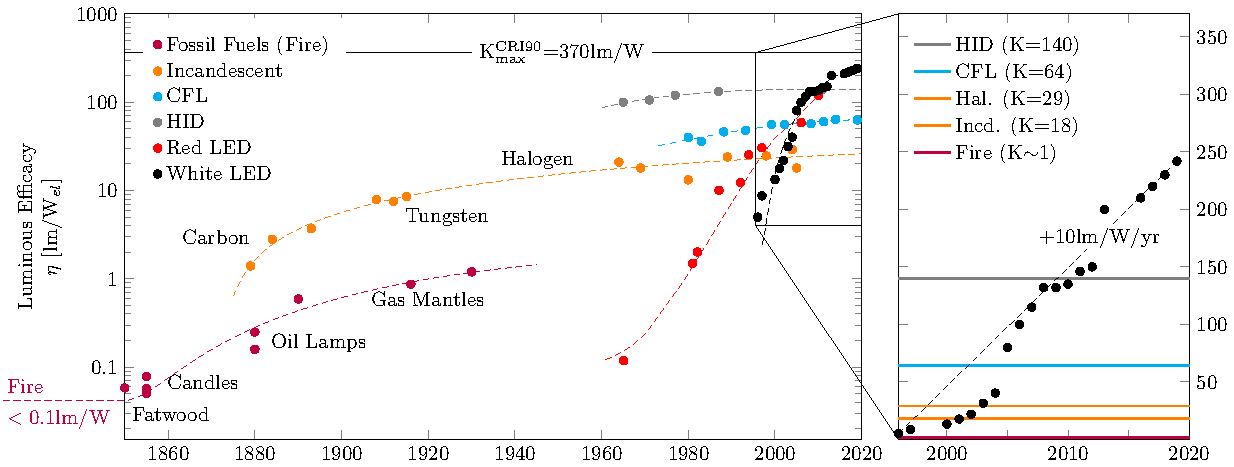
\includegraphics[width=\textwidth]{figures/history_efficacy.pdf}
 \caption{\textbf{Historical progress in the luminous efficacy ($\eta$) of the most widely-used lighting technologies in human history.} Data points indicate best performers by year of market introduction. Luminous efficacy is the measure of how efficiently a light source converts electrical energy into visible light that can be perceived by the human eye, taking into account the wavelength sensitivity of the eye (see Supplementary Note 2 for details). Dashed lines are guides to the eye, based on a 3rd-order polynomial fit to the data trend. The physical limit for an ideal light source with a colour rendering index of CRI=90, denoted as $K_{max}^{CRI90}$, is shown as a black horizontal line, as per calculations by Murphy et al. \cite{Murphy2012}. The magnified plot shows the progress in cool white LEDs from 1996 to 2020, with the dashed line indicating a linear rate of efficacy improvement of 10lm/W per year. For comparison, efficacies of best performers in legacy lighting technologies for 2020 are shown as coloured horizontal lines. Note the logarithmic scale of the vertical axis on the main plot and the linear scale on the magnified plot. Abbreviations: HID - High-Intensity Discharge; CFL - Compact Fluorescent Lamp; Hal. - Halogen, Incd. - Incandescent. Source: own synthesis of published data based on a visual approach proposed by Azevedo et al. \cite{azevedo2009transition}. See Supplementary Note 7 for the full list of sources and references.}
 \label{fgr:history_efficacy}
\end{figure}

\begin{figure}[h!]
\centering
  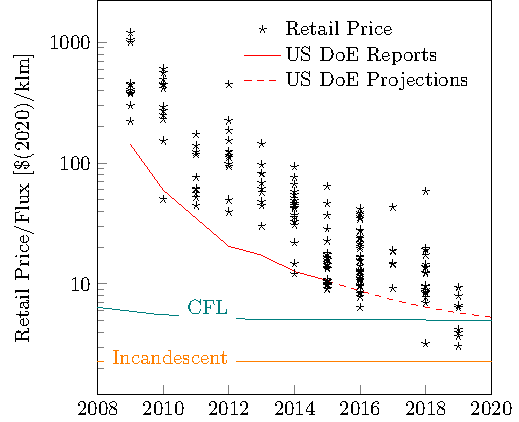
\includegraphics[height=6.5cm]{figures/cost_lamp_small.pdf}
  \caption{\textbf{Historical development of retail sales prices per luminous flux for LED-based luminaires in the period 2008-2020.} Luminaires considered include light bulbs, spotlights and recessed lights. Red curved and dashed lines represent average retail sales prices and price projections for LED based luminaires published by the U.S. Department of Energy (DOE) \cite{national2013assessment}. Shown for reference are the average prices for compact fluorescent (CFL) and incandescent light bulbs, with the latter assumed constant based on the average in the covered time period. Source: own synthesis of data on sales prices collected from various consumer watchdog databases and publications. See Supplementary Note 7 for the full list of sources and references.}
  \label{fgr:cost_lamp_small}
\end{figure}

These dramatic improvements in lighting technology, supported by the introduction of lighting efficiency regulations phasing out incandescent lightbulbs and targeted policies stimulating LED adoption in many countries, led to the rapid expansion and diffusion of SSL technologies \cite{weinold2020long, stegmaier2021incandescent, Mills2014}. As a result, by 2020, highly efficient LED luminaires were saving an estimated 131 TWh/year in the EU \cite{eu2019impactass} and 442 TWh/year for the US \cite{guidehouse2020adoption}, which is on par with the amount of energy produced annually by all solar photovoltaic installations in these regions. Notably, market adoption of LED lighting is not limited to developed economies \cite{Kamat2020}. For example, durability, low up-front cost and high efficiency of LED light sources have led to their widespread adoption in rural West African communities without access to grid electricity \cite{Bensch2017}. LEDs have also been used in a wide range of applications beyond lighting, such as personal health monitors \cite{Wyatt2020}, watches and smartphones \cite{Bai2017}, potable water treatment \cite{Lui2014}, high-bandwidth wireless data transmission \cite{Haas2016}, and augmented reality eye wear \cite{Lee2016}. 

Despite this impressive history, the sources of technological progress in white LEDs have not received as much attention from researchers as innovation  in supply-side energy technologies, such as solar photovoltaics \cite{kavlak2018evaluating, nemet2019solar}, wind energy \cite{qiu2012price, jennings2020policy}, or lithium-ion batteries \cite{Ziegler2021, Stephan2021}. To the best of our knowledge, no study has comprehensively discussed the sources or extent of historical progress across a range of metrics related to LED cost and performance since the introduction of the first commercial white LED products (see Supplementary Note 1 for a brief review of previous literature on this topic). This is consistent with previous observations regarding the marginalization of end-use technologies in the analysis of energy innovation for climate change impact mitigation \cite{Wilson2012, Creutzig2018}. Understanding the extent to which individual innovations and technology spillovers contributed to improvements in white LED technology, how their effect compares to other sources of improvements such as economies of scale, and how these innovations and spillovers occurred (i.e., by what mechanisms and actors) will provide valuable lessons for innovation in other demand-side energy technologies and clean energy innovation in general.

To address these questions, first, we identify three sets of metrics suitable for tracking the historical progress of LED lighting technology: 1) metrics of energy efficiency of LED devices, including the total device efficiency (“lamp efficiency”) and the sub-efficiencies that describe different energy loss channels in a LED device; 2) metrics of lighting quality relevant to consumer experience, including colour rendering index (CRI) and colour temperature (CT); and 3) LED device manufacturing cost. The rationale for the choice of these metrics, along with their detailed descriptions and definitions, are discussed in Supplementary Note 2. We then trace the historical improvements in these metrics, along with associated changes in LED chip architectures, from the time of introduction of the first commercial warm white GaN-based LEDs in 2003 to 2020, the year with the most recent data available at the time of data collection. Given the proprietary nature of knowledge in the SSL industry, we collect corresponding information using a multi-method approach combining a comprehensive review of scientific literature and industry reports with patent analysis and a series of elite interviews \cite{tansey2009process} with eminent experts from academia, public research institutions and industry (see Methods section and Supplementary Note 3 for details). This approach allows us to identify individual innovations in white LED technology, examine their knowledge origins to discern technology spillovers among them and quantify their contributions to the overall progress in LED efficiency and consumer experience metrics based on our modeling of LED performance and spectral metrics. We further develop a bottom-up LED manufacturing cost model with process-step resolution and use it to analyze the progress in LED manufacturing cost for the “classical” GaN-based LED chip architecture with lateral current spreading shown in Panel A in \cref{fgr:chip_architecture_overview}.

\section{Main}

% should be integrated into some other sub-heading
% \subsection{Evolution of LED Chip Architectures}

\clearpage
\begin{figure}[h!]
\centering
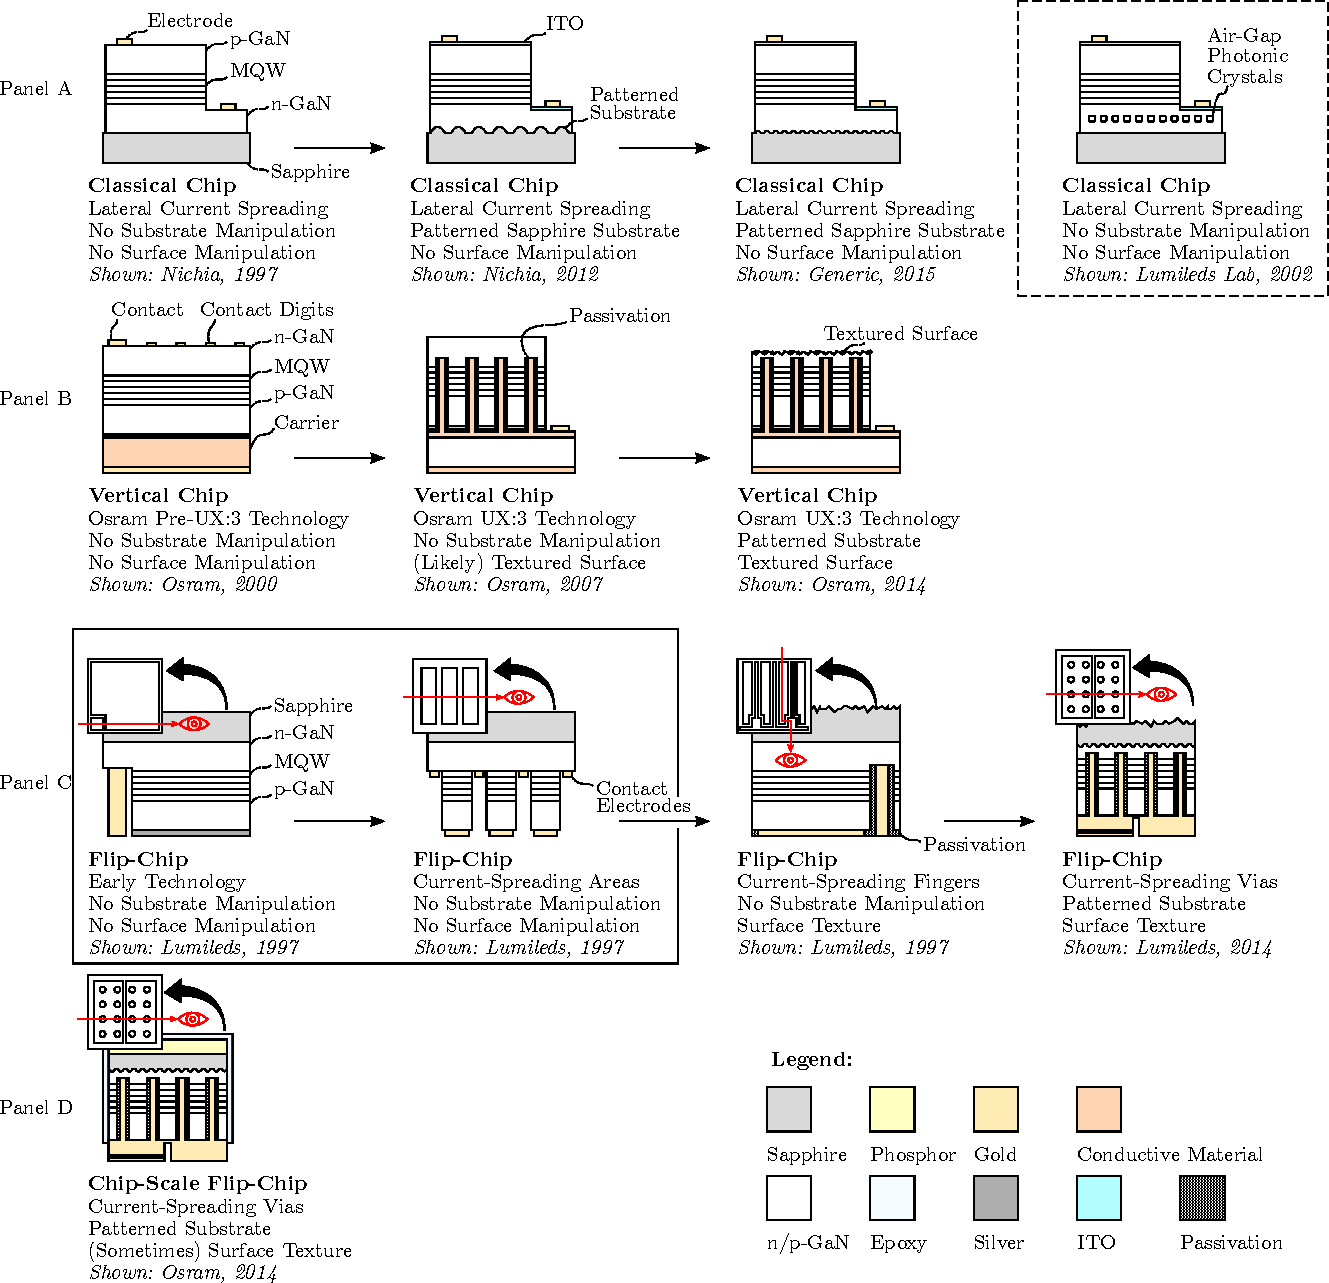
\includegraphics[height=15cm]{figures/chip_architecture_overview.pdf}
\caption{\textbf{Historical evolution of LED chip architectures.} Panel A: classical chip with lateral current spreading; Panel B: Osram’s thin GaN flip-chip (vertical) architecture; Panel C: flip-chip architecture; Panel D: chip-scale package flip-chip architecture. Shown are side views of chips without packages, along a cutaway line best suited to the features of each architecture. The cutaway surface is indicated by a red arrow with an eye on the overlaid top view of each chip. Note that the dimensions are not to scale, and smaller features are greatly exaggerated for clarity. Years indicated correspond to the earliest identified patent priority date. Black frames around certain designs indicate chip designs not brought to large-scale production. Chip architecture abbreviations: TF - Thin-Film; FC - Flip-Chip; CSP - Chip-Scale Package; Material abbreviations: GaN - Gallium Nitride, ITO - Indium Tin Oxide, MQW - Multiple Quantum Well. Source: adapted and compiled from multiple patents and industry publications. See Supplementary Note 7 for the full list of sources and references.}
\label{fgr:chip_architecture_overview}
\end{figure}

We summarize the information collected and analysed on the progress in GaN-based LED chip architectures and manufacturing processes in \cref{fgr:chip_architecture_overview}, where we show the evolution of LEDs from classical chips with lateral current spreading to chip-scale package flip-chip architectures. We use this information as input into LED performance calculations and manufacturing cost modeling. 

\subsection{Efficiency Improvements}

The historical progress in individual sub-efficiencies of warm white phosphor-converted GaN-based LED devices, along with LED innovations and manufacturing process improvements that have driven this progress, is described in Supplementary Note 4. Using this information, we calculate the overall lamp efficiency $\eta_L$ for the best performing mid/high-power phosphor-converted warm white LED devices in four years: 2003, 2010, 2016 and 2020. The waterfall diagrams of electric power input losses in \cref{fgr:waterfall} show how improvements in individual sub-efficiencies led to improvements in the overall white LED lamp efficiency from $\eta_L=5.8\%$ in 2003 to 12.7\% in 2010, 32.5\% in 2016 and finally to 38.8\% in 2020. As is evident from the figure, no single loss channel dominates in terms of its contribution to the overall efficiency, in line with previous observations \cite{tsao2010solid}. We note, however, that the loss channels with a fixed physical limit on efficiency, e.g., Stokes loss that determines the light conversion efficiency by phosphors, became relatively more dominant in 2016 and 2020 compared to 2003 and 2010.  This is a direct result of large efficiency improvements in upstream sub-efficiencies.

\cref{fgr:breakthroughs_efficiency} shows the overall magnitude of contributions of identified LED innovations and technology spillovers to improvements in LED efficiency over time across different sub-efficiencies. The full list of identified LED innovations considered in our study is provided in Table SI2 in Section 3 of the Supplementary Information document. The list of corresponding technology spillovers is provided in \cref{tab:spillovers} in the Discussion section below. Through the index decomposition analysis described in Section 2.5 in the Supplementary Information we find that out of the overall LED efficiency increase of 32.9\% from 5.8\% to 38.8\% between 2003 and 2020, at least 2.8\% can be attributed specifically to technology spillovers identified in this study, corresponding to 8.5\% of the total LED efficiency improvements between 2003 and 2020.

In \cref{fgr:breakthroughs_efficiency} we also compare, for the first time, efficiency improvements across sub-efficiencies over time, contrasting them with the physical limits of the corresponding loss channels. We find that there has been consistent progress across all device sub-efficiencies in the recorded period. Specifically, between 2003 and 2020, forward voltage efficiency increased from 70\% to 99.5\%, internal quantum efficiency from 55\% to 90\%, electrical droop from 65\% to 90\%, light extraction efficiency from 60\% to 90\%, spectral efficiency from 74\% to 83\%, conversion efficiency (red) from 11\% to 45\%, conversion efficiency (green) from 19\% to 61\%. Notably, some sub-efficiencies for the most recent devices considered in our study are now within $\sim10\%$ of their respective physical limits. The exception is spectral efficiency which, at $\sim17\%$ below the physical limit, shows larger potential for further improvements, which is important, given that efforts to improve LED performance across different efficiency loss channels through R\&D continue \cite{cho2017white, Weisbuch2020}. 

\begin{figure}[H]
 \centering
 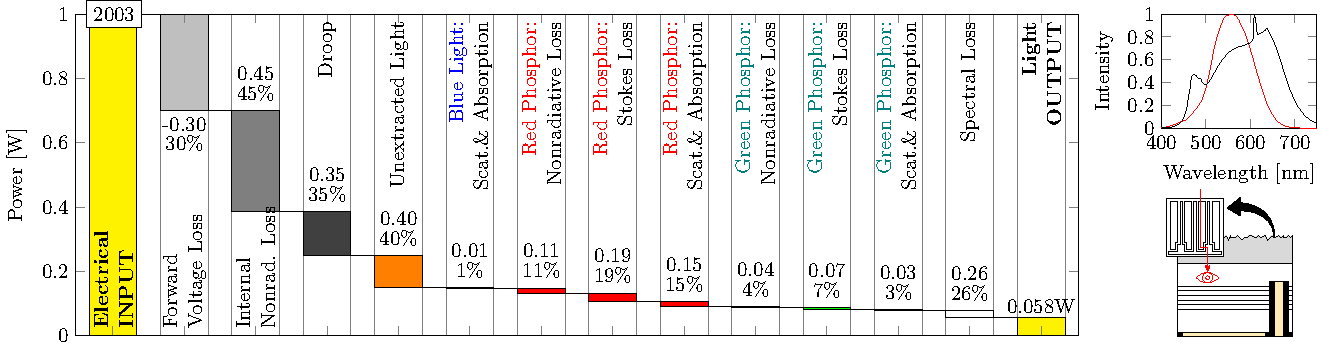
\includegraphics[width=15.5cm]{figures/waterfall_performance_2003.pdf}
 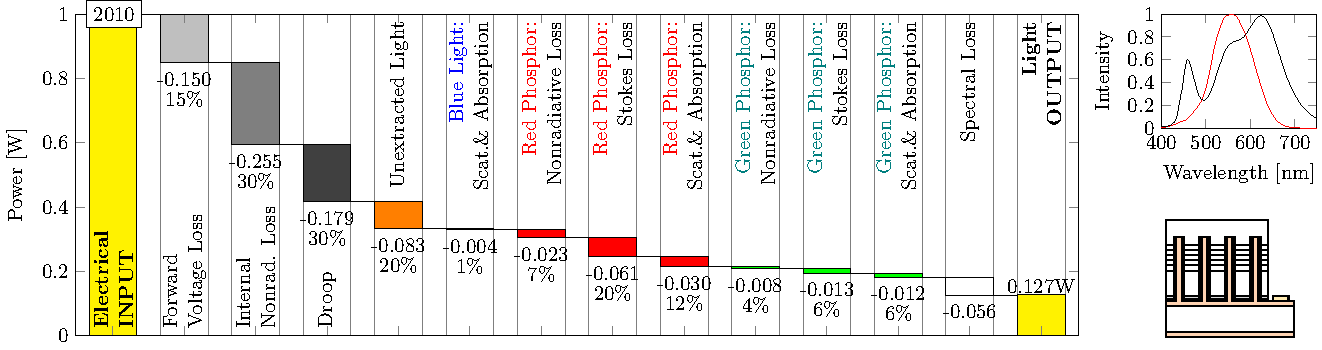
\includegraphics[width=15.5cm]{figures/waterfall_performance_2010.pdf}
 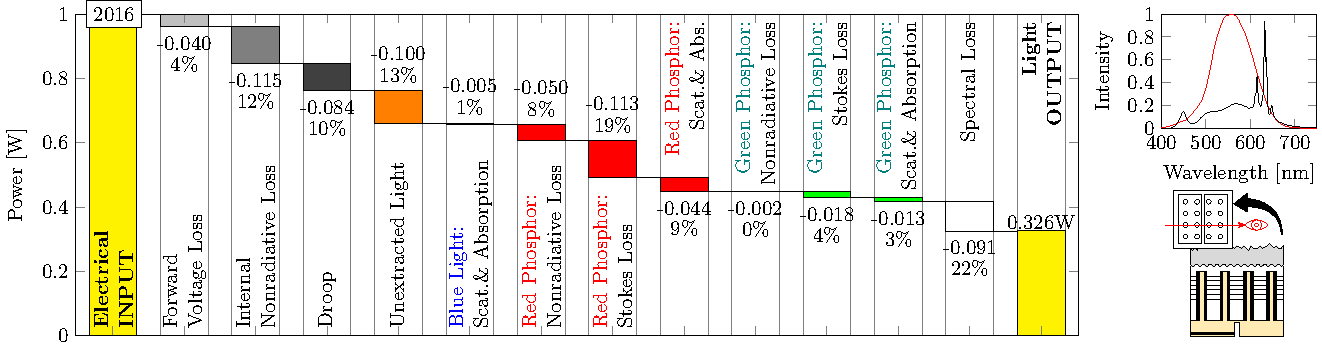
\includegraphics[width=15.5cm]{figures/waterfall_performance_2016.pdf}
 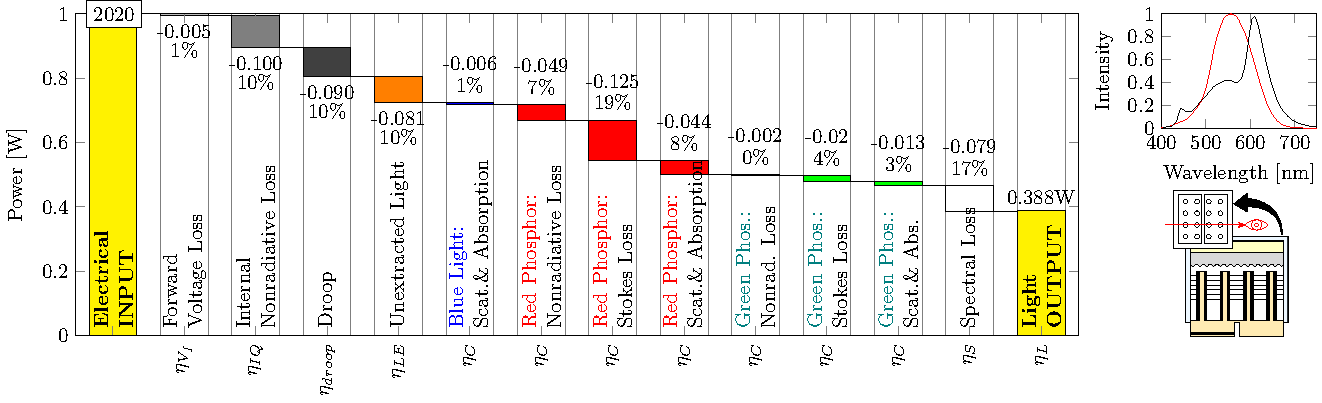
\includegraphics[width=15.5cm]{figures/waterfall_performance_2020.pdf}
 \captionsetup{font=footnotesize}
 \caption{\textbf{Waterfall diagrams of the loss channels in a generic mid/high-power LED package for 2003, 2010, 2016 and 2020}. Losses are normalized to 1 Watt of electric power input (yellow bar on the left). Sub-efficiencies corresponding to each loss channel are listed below each column and described in Supplementary Note 2.  Numbers for each loss channel indicate energy losses both in relative terms of input power (in percent) at the point of the channel and absolute values (in Watts). Percentages for loss channels labeled by red, green and blue font indicate losses of corresponding remaining red/green/blue light energy. The following LED architectures and down-conversion phosphor spectra used in calculations in each considered year are shown for reference: 2003 – Flip-chip with YGAG phosphor; 2010 – Flip-chip with 258 phosphor; 2016 – Flip-chip with PFS phosphor; 2020 – Chip-scale package flip-chip with SALON phosphor. Details for each architecture are provided in \cref{fgr:chip_architecture_overview}.  Details on the phosphors for light down conversion are provided in \cref{tab:phosphors} and Supplementary Note 4. Abbreviations: Scat. = Scattering; Nonrad. = Nonradiative. Source: own elaboration based on data on sub-efficiencies presented in Supplementary Figure 9 and spectral data in Supplementary Figure 10, adapted from publications on the respective phosphors: YGAG (2003)\cite{Mueller2002}, 258 (2010)\cite{MuellerMach2005}, PFS (2016)\cite{Murphy2015}, SALON (2019)\cite{Hoerder2019}.}
 \label{fgr:waterfall}
\end{figure}

\begin{figure}[H]
 \centering
 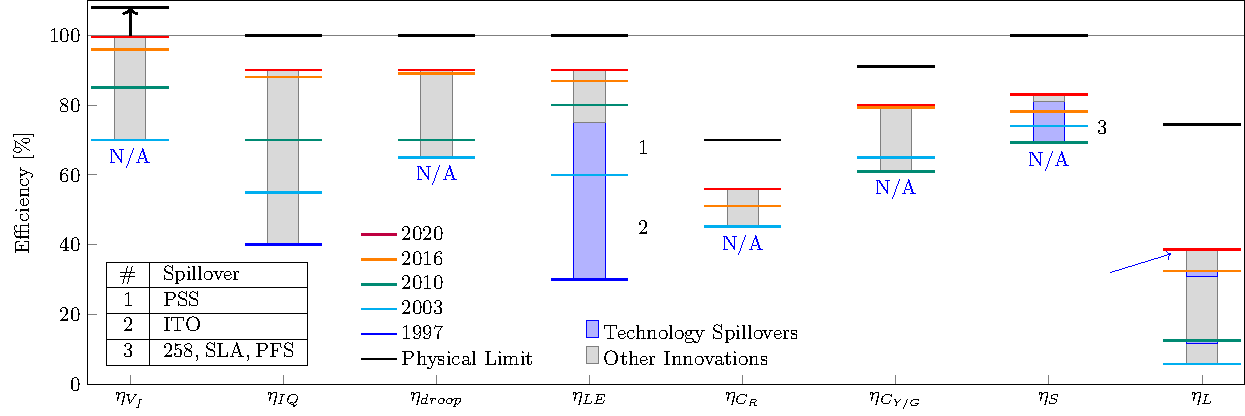
\includegraphics[width=\textwidth]{figures/breakthroughs_efficiency.pdf}
 \caption{\textbf{Contribution of innovations and technology spillovers to the historical progress in sub-efficiencies of phosphor-converted warm white LEDs.} LEDs with test currents of at least 350mA are considered. The following sub-efficiencies are represented: $\eta_{V_f}$ - forward voltage efficiency; $\eta_IQ$ - internal quantum efficiency; $\eta_{droop}$ - efficiency droop; $\eta_{LE}$ - light extraction efficiency; $\eta_{C_R}$ - conversion efficiency for red phosphors; $\eta_{C_{Y/G}}$ - conversion efficiency for yellow/green phosphors; $\eta_S$ - spectral efficiency. The overall LED lamp efficiency $\eta_L$ is displayed in the rightmost column. Vertical bars represent cumulative contributions to efficiency improvements from LED technology innovations, with purple bars indicating innovations driven by technology spillovers (annotated and listed in an inset table) and grey bars indicating all other improvements identified in this study. Horizontal coloured lines indicate sub-efficiency levels of best performing LEDs for the four years used in \cref{fgr:waterfall}: 2003, 2010, 2016, and 2020. For additional historical context, data for 1997 is included whenever possible. "N/A" denotes sub-efficiencies where 1997 data could not be calculated for the following reasons: $\eta_{V_f}, \eta_{droop}$ depend on the device current, which was below 350mA in 1997, making a comparison with contemporary devices difficult. $\eta_{C_R}, \eta_{C_{Y/G}}$ and $\eta_S$ are relevant only to warm white spectrum LEDs, which were not available in 1997. Note: ITO current spreading layer affects different sub-efficiencies in different chip architectures, e.g., in modern flip-chip architectures $\eta_{LE}$ no longer depends on ITO, see \cref{fgr:chip_architecture_overview}. Physical limits on sub-efficiencies are indicated by black horizontal lines. Note that the physical limit of $\eta_{V_f}$ is above 100\% due to quantum effects \cite{david2016electrical}. Source: own elaboration based on data represented in \cref{fgr:waterfall}, \cref{tab:spillovers} and Supplementary Note 4.}
 \label{fgr:breakthroughs_efficiency}
\end{figure}

\subsection{Consumer Experience Improvements}

Historical improvements in consumer experience metrics for phosphor-converted warm white GaN-based LEDs are shown in \cref{fgr:consumer_experience}. In general illumination applications, a high colour rendering index (CRI) in combination with a specific, tunable range of possible colour temperatures is desirable. Both metrics are determined by LED device emission spectra, which, in turn, depend on the properties of materials used for the conversion of blue light generated by conventional GaN-based LEDs into the white light required for general illumination . It allows us to establish the links between all major improvements in the two consumer experience metrics considered in this study and individual LED innovations  associated either with phosphors or quantum dots used for light down conversion in LEDs. The first commercial white LED produced by Nichia in 1996 used a YAG (Yttrium Aluminium Garnet) phosphor that could generate only cool white light \cite{bando1998development}. As shown in \cref{fgr:consumer_experience}, after a series of innovations listed in \cref{tab:phosphors}, LEDs today can be tuned for high CRI performance and a range of desirable colour temperatures.  

Notably, from detailed descriptions of the history of innovations in this list, provided in Supplementary Note 4, we find that only a single innovation related to LED consumer experience improvements was initially intended exclusively for application in solid-state lighting: the 2016 SALON phosphor compound \cite{Hoerder2019,seibald2019phosphor}. All other innovations in the list were either originally developed for non-LED applications or prominently used knowledge from areas of science and technology beyond LED or SSL (see also \cref{tab:spillovers}). This means that technology spillovers contributed to nearly all consumer experience improvements in LED-based lighting technology, thus playing an important role in widespread adoption of SSL in general illumination applications. 

\begin{table}[H]
    \footnotesize
    \centering
    \caption{\textbf{LED innovations related to improvements in consumer experience metrics.}}
    \begin{NiceTabularX}{\textwidth}{|l|l|l|X|X|l|}
    \hline
        \textbf{Year} & \textbf{Desig.} & \textbf{Chemical formula} & \textbf{Description} & \textbf{Significance} & \textbf{Ref.} \\ \hline
        1996 & YAG & $Y_3 Al_5 O_{12}:Ce$ & Yttrium aluminium garnet (YAG) phosphor activated with cerium & First LED phosphor, enabled white LEDs & SI 3.2.2.1 \\ \hline
        1996 & YGAG & $(Y_{1-x} Gd_x)_3 Al_5 O_{12}:Ce$ & Gadolinium-doped YAG phosphor & First red-shifted phosphor, enabled warm white LEDs & SI 3.2.2.1 \\ \hline
        2002 & 258 & $(Ba,Sr)_2 Si_5 N_8:Eu^{2+}$ & Europium-doped nitridosilicate phosphor & First red LED phosphor & SI 3.2.2.2 \\ \hline
        2003 & QD & N/A & Quantum dot-based phosphor & First use of QD for LED light down conversion & SI 3.2.2.4 \\ \hline
        2005 & PFS & $K_2 SiF_6: Mn^{4+}$ & Manganese-activated potassium fluorosilicate (PFS) phosphor & First ultra-narrow-band red LED phosphor & SI 3.2.2.3 \\ \hline
        2013 & SLA & $Sr[Li Al]_3 N_4 ]:Eu^{2+}$ & Europium-doped cuboidal nitridolithoaluminate phosphor & Improved narrow-band red phosphor & SI 3.2.2.2 \\ \hline
        2016 & SALON & $Sr[Li_2 Al_2 O_2 N_2]:Eu^{2+}$ & Europium-doped oxonitride phosphor & High-performance ultra-narrow-band red phosphor & SI 3.2.2.2 \\ \hline
    \end{NiceTabularX}
    \caption*{Note: \textit{Year} column represents the earliest reported application of innovation in white LEDs. These differ from the years shown in \cref{fgr:consumer_experience} which correspond to the earliest publication of spectral data for LED products that relied on those innovations. Detailed descriptions of the history of each innovation and relevant spectral data are provided in Supplementary Note 4. Desig.=Designation, Ref.=Reference.}
    \label{tab:phosphors}
\end{table}

\begin{figure}[H]
 \centering
 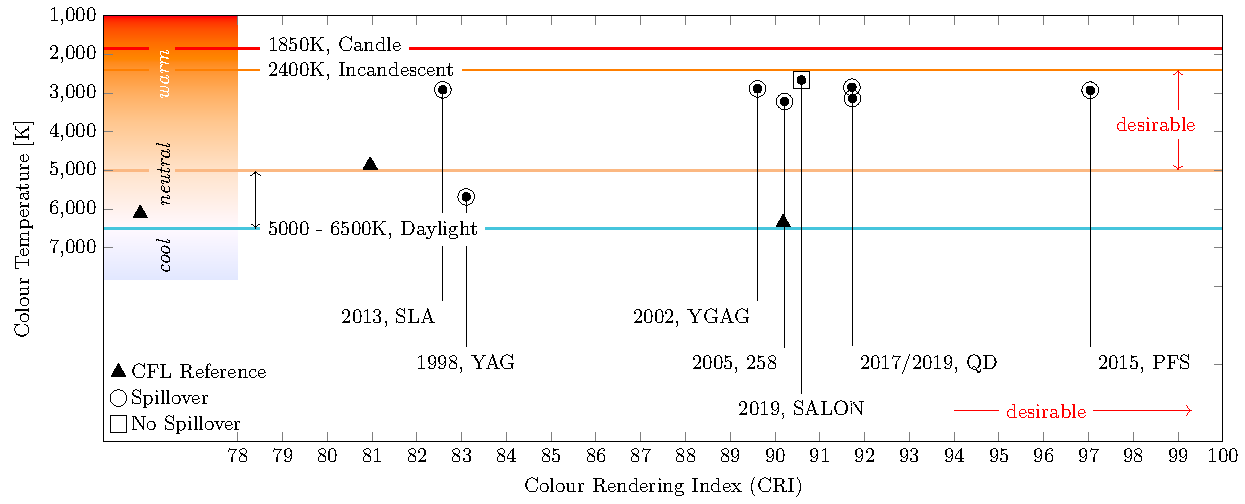
\includegraphics[width=\textwidth]{figures/breakthroughs_consumer-experience.pdf}
 \caption{\textbf{Historical improvements in consumer experience metrics of phosphor-converted white LEDs.} Data points show the color temperature (CT) and colour rendering index (CRI) performance of the earliest identified representative white LED products with published spectral data that used phosphors listed in \cref{tab:phosphors}, each indicated by the phosphor label and publication year. Corresponding spectral data used to calculate CT values is provided in Supplementary Note 4. Three data points representing compact fluorescent lamps (CFLs)\cite{cie_reference}, shown as black triangles, are provided for comparison. Horizontal lines represent typical CTs of “traditional” light sources, shown for reference. The desirable range of colour temperatures for home illumination, indicated by a vertical red arrow, lies between two horizontal orange lines representing typical incandescent light and warm daylight colour temperatures. Horizontal red arrow indicates desirable higher values of colour rendering index (CRI). LED products based on the following phosphor innovations from the following LED manufacturers are represented : YAG - Nichia, 1998 \cite{bando1998development}; YGAG - Lumileds, 2002 \cite{Mueller2002}; 258 - Lumileds, 2005 \cite{MuellerMach2005}; SLA - Lumileds, 2014 \cite{Pust2014}; PFS - GE, 2015 \cite{Murphy2015}; QD - Lumileds, 2017 \cite{lumileds2016qd}, Osram, 2019 \cite{osram2019qd}; SALON - Osram, 2019 \cite{Hoerder2019}.}
 \label{fgr:consumer_experience}
\end{figure}

\subsection{Manufacturing Cost Improvements}

\cref{fgr:costmodel} shows main results of our manufacturing cost modelling for low-to-mid-power classic chip GaN phosphor-converted white LED packages. We find that the manufacturing cost of a single such LED decreased from 1.11\$ (in 2020 USD) in 2003 to 0.11\$ (2020 USD) in 2012 and 0.05\$ in 2020, a 95.5\% overall decrease. Our model shows that for the wafer-level manufacturing steps illustrated in Supplementary Figures 2-6, yield improvements and an increase in  wafer size together are responsible for a 98\% reduction of manufacturing cost per LED chip between between 2003 and 2020.

Among the factors contributing to the LED cost reductions over time, improved manufacturing yields and increases in the wafer size rather than particular LED innovations are found to be responsible for the largest contribution to the overall cost reduction. In the case of manufacturing yield, the higher it is, the less inputs are wasted on the production of a single LED package. With the total manufacturing yield dramatically improving from $\sim25\%$ in 2003 to $\sim75\%$ in 2020 (compare \cref{fgr:costmodel}, Panel D), it is not surprising that the total yielded LED manufacturing cost significantly declined over this period.

In the case of wafer diameter, the larger the wafer, the more LED chips can be produced from a single wafer. The wafer diameter commonly used in LED manufacturing has been steadily increasing from 50mm ($\sim2$ inch\footnote{Industry measures wafer size in mm. Still, a 50mm=1.9685Inch wafer is frequently referred to as a "2-inch wafer".}) in 2003 to 200mm ($\sim$8 inches, referred to as “8 inch") in 2020. We capture this effect in the model by calculating the associated number of die per wafer (DPW) for each representative wafer diameter d \cite{de2005investigation}: $d(2003)\sim 50 mm \rightarrow851 DPW$, $d(2020)\sim200 mm \rightarrow 26,838 DPW$ (see Supplementary Figure 7 in Supplementary Note 3). With more than a thirty-fold increase in the number of die per wafer between 2003 and 2020, the contribution of the whole-of-wafer processing steps to the total cost of manufacturing an individual LED chip and package has dramatically declined over time. As the number of die per wafer increases, the packaging steps, which in the classic chip architecture must be performed separately for each individual LED chip, carry a significantly larger share of the total cost in 2020 than in 2003 (compare Panels A-C in \cref{fgr:costmodel}). However, as our interviewees noted, while growing LEDs on larger wafers is economically desirable, it is associated with engineering and epitaxy challenges as well as high up-front cost of new equipment.

Our findings are further supported by a preliminary sensitivity analysis, presented in Section 5 of the Supplementary Information section, where we find that the sensitivity of the cost model to variation in its main parameters decreases over time with the increase of the number of DPW. 

In Supplementary Note 6, we also provide a comparison of the outcomes of our model with past cost calculations and projections published by the U.S. Department of Energy (DOE) on the basis of the \textit{LEDCOM} cost model \cite{ledcomv2} and industry data reported to the DOE as part of SSL round tables.

\begin{figure}[ht!]
\centering
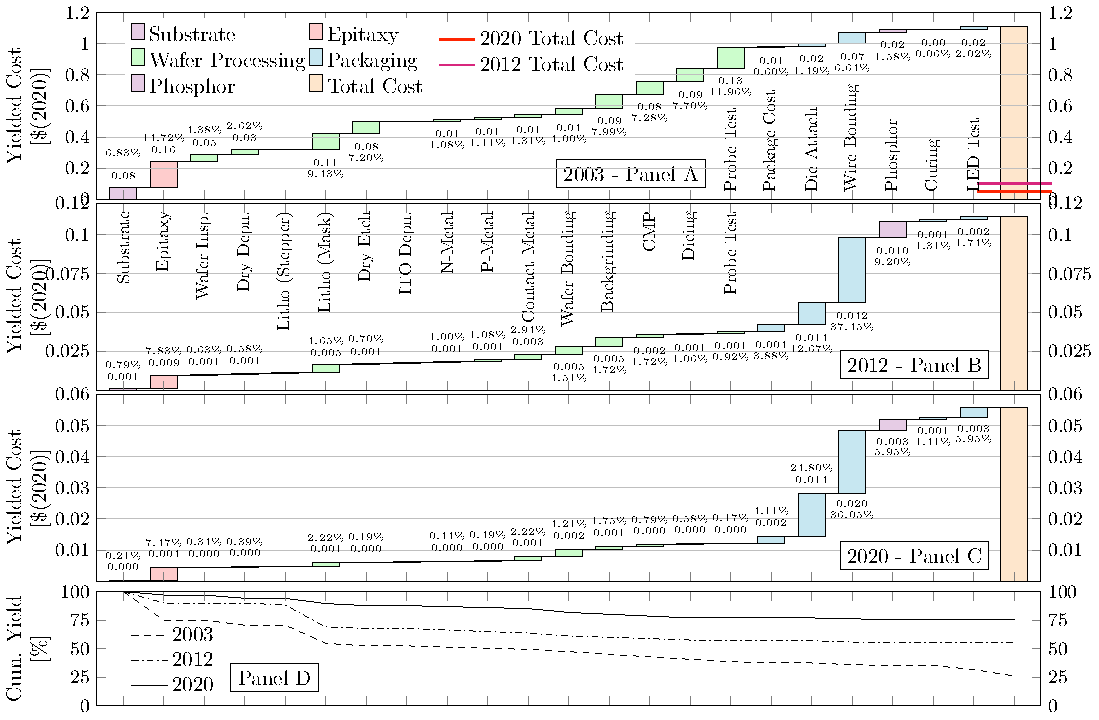
\includegraphics[width=17.5cm]{figures/costmodel_results_years.pdf}
\caption{\textbf{Historical changes in LED manufacturing cost structure.} Presented cost calculations are an outcome of our cost model (see \cref{sec:methods} and Supplementary Note 3) for a single low-to-mid power GaN-based, classic chip, phosphor-converted white LED package, assuming an ideal factory with state-of-the-art equipment at a U.S. location. Panels A-C: Waterfall diagrams of LED manufacturing cost structure split by manufacturing process steps for years 2003, 2012 and 2020. Process steps on the horizontal axis are sequenced from left to right in the same order as in the modelled LED manufacturing process. Panel D: Cumulative manufacturing yield after each process step for years 2003, 2012 and 2020. For a graphic representation of the manufacturing process, see the diagrams in Supplementary Figures 2-6. Abbreviations: Litho – Lithographic Process, Insp. – Inspection, Depn. – Deposition, CMP - Chemical-Mechanical Planarization.}
\label{fgr:costmodel}
\end{figure}

\subsection{Technology Spillovers}

Following the frameworks for the analysis of technology spillovers proposed by Stephan and colleagues \cite{Stephan2021} and Kolesnikov et al. \cite{kolesnikov2022technology}, we synthesize information from the interviews, historical records, literature review and citations in patents and publications to identify which LED innovations involved knowledge originating in areas of science and technology beyond LED and SSL. We find that at least nine LED innovations, listed in Table 2, clearly involved such ‘external’ knowledge. We then analyze the sources, mechanisms and enablers of corresponding technology spillovers, as well as their contributions to progress in white LED technology. 

We find that three spillovers associated with the use of YAG/YGAG phosphors in LEDs played the key role in the development of the first commercial white LED lighting products, essentially enabling the solid-state lighting market and industry of today. As noted above, subsequent spillovers then had a significant effect on physical device performance, cumulatively contributing to 8.5\% of the total LED lamp efficiency improvements between 2003 and 2020, as well as nearly all key improvements in consumer experience metrics.

Among the spillover sources, we find that all nine spillovers had origins in the scientific disciplines such as various branches of chemistry, materials science, optics and photonics, and solid-state physics. Five spillovers also utilized technical knowledge and expertise in cathode ray tubes, fluorescent lighting, optoelectronic devices, nanotechnology, and nature-inspired material design.
Among the spillover mechanisms, six spillovers (involved in all phosphors except PFS and SLA, plus ITO) were a result of application of external scientific and technical knowledge already available to researchers and inventors. Three remaining spillovers (involved in PFS and SLA phosphors, plus PSS) occurred as an outcome of targeted search for relevant external knowledge outside the LED domain. In addition, at least two spillovers (involved in 258 and PFS phosphors) occurred as a result of knowledge exchange in direct R\&D collaboration.

Among important enabling factors for the identified spillovers, we highlight public mission-driven R\&D funding; industry-academia partnerships; firm experience in multiple industries; conferences that brought together researchers from academia and industry; cultural and language proximity; freedom of search in academia; and university alumni networks.
Finally, we find that, on average, it took 26 years from the initial scientific discovery or invention to the moment of its spillover into the LED domain, with this time varying from 5 to almost 70 years. In contrast, it took much less time – just 6 years on average, varying from just a few months to 19 years – to develop a commercial application for the spillover knowledge in the LED market.

\begin{table}[h!]
    \tiny
    \centering
    \caption{\textbf{Technology spillovers involved in white LED technology innovations identified in this study.}}
    \begin{NiceTabularX}{1.1\textwidth}{|l|l|l|X|X|X|X|X|X|}
    \hline
        \textbf{Disc.} & \textbf{S/O} & \textbf{Comm.} & \textbf{LED Innovation} & \textbf{Spillover} & \textbf{Enabler} & \textbf{Origin} & \textbf{Ref.} & \textbf{Area of Improvement} \\ \hline
        1926 & 1994 & 1996 & LED phosphors &  Use of phosphors for light down conversion in LEDs & ??? & Materials science (S), Cathode ray tubes (T) & \cite{bright1972electric,shimizu1994sheet,cho2017white} & Enabled light down conversion in LEDs \\ \hline
        1967 & 1996 & 1996 & YAG phosphor & Use of YAG phosphor in a first white LED product & ??? & Chemistry (S), Materials science (S), Fluorescent lighting (T), Cathode ray tubes (T) & \cite{blasse1967new,bando1996,bando1998development,shimizu1999light,cho2017white} & Enabled white LED products, $\eta_S$, $\eta_C$ \\ \hline
        1967 & 1996 & $<$2002 & YGAG phosphor & Use of YGAG phosphor in first warm white LEDs & ??? &  Chemistry (S), Materials science (S) & \cite{holloway1969optical,bando1998development,shimizu1999light,Mueller2002} & Enabled warm white LEDs, $\eta_S$, $\eta_C$ \\ \hline
        1982 & 1996 & $<$2010 & Patterned sapphire substrate (PSS) & Use of anti-reflective properties of substrate patterns in LEDs & targeted search & Optics and photonics (S), Materials science and technology (S,T), Nature-inspired material design (T)  & \cite{moharam1982diffraction,krames1998ordered,feezell2018invention,Narukawa_2010} & $\eta_{LE}$, $\eta_{IQ}$ (depending on the chip architecture, compare \cref{fgr:chip_architecture_overview})\\ \hline
        1971 & 1999 & $<$2005 & Indium tin oxide (ITO) current spreading layer & Use of ITO current spreading layer in white LEDs & targeted search & Optics and photonics (S), Materials science and technology (S,T), Optoelectronic devices (T) & \cite{vossen1971rf,fraser1972highly,margalith1999indium} & $\eta_{Vf}$, $\eta_{LE}$ (depending on the chip architecture, compare \cref{fgr:chip_architecture_overview}) \\ \hline
        1997 & 2002 & 2005 & 258 phosphor & Use of luminescent ‘258’ nitridosilicate compound as LED phosphor & research conference & Chemistry (S), Materials science (S) &\cite{Huppertz1997,mueller2004phosphor,MuellerMach2005} & $\eta_S$, $\eta_C$ \\ \hline
        1984 & 2003 & 2009 & Quantum dot-based phosphor & Use of quantum dots for light down conversion in LEDs & ??? & Solid-state physics (S), Photochemistry (S), Nanotechnology (T) &\cite{fojtik1984photo,simmonsfinal,ledprof_nexxusqd,bourzac2013quantum} & $\eta_S$, $\eta_C$ \\ \hline
        1972 & 2005 & 2015 & PFS phosphor & Use of knowledge in luminescent materials and skills in "wet" chemical synthesis to synthesize PFS compound and optimize it as LED phosphor & ??? & Chemistry (S), Materials science (S) &\cite{paulusz1973efficient,radkov2009red,Murphy2015} & $\eta_S$, $\eta_C$ \\ \hline
        2008 & 2013 & 2015 & SLA phosphor & Use of knowledge about existing cuboidal nitride compounds to identify and synthesize structurally similar SLA phosphor & ??? & Structural chemistry (S), Materials science (S), Solid-state physics (S) &\cite{Park2008New,schmidt2013new,Pust2014} & $\eta_S$, $\eta_C$ \\ \hline
    \end{NiceTabularX}
    \caption*{Note: Disc. - Year of initial discovery, identified  by the earliest literature source describing the discovery of original idea or invention outside the LED domain. S/O - Year of spillover to LED; Comm. - Year of commercial application, identified as the year of the first recorded application of that idea or invention in a commercial LED product. Ref. - References. LED innovations are ordered by the year in which a technology spillover into LED occurred, provided in the S/O column. Origin column represents knowledge domains in which spillovers initially emerged, where (S) denotes a scientific discipline and (T) is an area of technology. Ref. column lists literature sources for the represented discoveries, innovations and spillovers. Area of Improvement column represents the impact of spillovers on different aspects of white LED technology, e.g., improvements in particular sub-efficiencies.}
    \label{tab:spillovers}
\end{table}

\section{Discussion}
\label{sec:discussion}

In this study, we use a multi-method approach to synthesize evidence from multiple sources and, for the first time, reconstruct a comprehensive picture of the rapid technological progress in white LED technology throughout its history since the introduction to the market in 1996 and across an ensemble of metrics related to device performance, cost, and consumer experience. Improvements in these metrics are traced to sources in innovation, technology spillovers, and economies of scale in the manufacturing process.

We find that the total LED device efficiency increase from 5.8\% to 38.8\% between 2003 and 2020, as well as all major improvements in consumer experience metrics, have been predominantly driven by LED technology innovations that reduced energy losses across all physical loss channels in LED devices and introduced new phosphor materials for LED light down conversion.  Our interviews have also revealed an important role of incremental manufacturing process improvements and learning-by-doing \cite{WRIGHT_1936, Arrow_1962} in the progress in LED efficiency. However, further research is needed to quantify the contribution of learning-by-doing to this progress. 

Our LED manufacturing cost model shows a 95.5\% decrease in the cost of producing low-to-mid power GaN-based white classic-chip LEDs from 1.11\$ to 0.05\$ (in 2020 USD) between 2003 and 2020. In contrast with LED performance improvements, where progress was driven mostly by innovations in LED technology, the dramatic decline in LED manufacturing cost has been a product of higher yields across manufacturing steps and economies of scale resulting from increases in the sapphire wafer size. 

Surprisingly, LED innovations and associated technology spillovers are not found to have a substantial impact on LED manufacturing cost reductions over time. There are several explanations for this finding. First, the functional unit of our study is the LED chip itself, not the luminaire containing multiple chips. As LED efficiency and overall brightness have increased, a smaller number of chips can be used in luminaires to obtain the same level of the overall light flux. However, since we are investigating improvements at the level of single chips, we do not capture the cost effects downstream of chip manufacturing. We also previously showed that overall brightness is no longer a target metric in chip development \cite{weinold2021compound}.

Second, we find that an increase in wafer size and higher overall yield, taken together, are jointly responsible for a 98\% reduction of manufacturing cost per LED chip between between 2003 and 2020. Both were enabled by advances in manufacturing equipment (e.g., for epitaxy and chip dicing) and incremental manufacturing process improvements from learning-by-doing, rather than particular LED innovations, which was confirmed by interviews with experts in LED manufacturing. 

Notably, our bottom-up cost model is constructed to provide process-step resolution across three different key chip architectures: classical chips, flip chips, and chip-scale package flip chips. However, in this study we were able to collect data and compare the outcomes only for the classical chip architecture. Collecting the full set of data needed to populate the model for the remaining two architectures requires access to proprietary information from industry. With this limitation, tracking manufacturing cost reductions across all three key LED chip architectures remains a topic for future work.

We find that technology spillovers into white LED technology have been significant drivers of improvements in LED efficiency and, particularly, consumer experience metrics. Our analysis of the sources, mechanisms and enablers of the identified technology spillovers has important practical implications, highlighting the critical role played by a deep understanding of the physical, chemical and optical phenomena underlying the operation of LEDs, as well as materials science and technology and nanotechnology involved in the production of LEDs, for past and future advances in LED and solid-state lighting technology. Specifically, deep physical understanding of LED device energy loss channels had enabled important innovations in LEDs that increased several sub-efficiencies in LEDs and will continue to do so, as expected by eminent experts in the field . This suggests that additional research in these areas and a more deliberate search for relevant external knowledge may accelerate expected future advances in LED technology and its applications both in SSL and technology areas beyond general illumination. Corresponding knowledge spillovers can be enabled and deliberately stimulated by various measures such as knowledge exchange events and long-term partnerships between academia and industry, interdisciplinary training and hiring, dedicated mission-driven public R\&D funding, and ensuring certain freedom of search in academia. These observations also further reinforce broader arguments made against the dichotomy of basic and applied research \cite{narayanamurti2016cycles, narayanamurti2021genesis} and the calls for open, inclusive and flexible research cultures \cite{Stephan2021}.

Finally, the lessons learned about the drivers of innovation, technology spillovers, cost reductions and performance improvements in LEDs may have broader implications both for other demand-side or energy-efficiency technologies, and for low-carbon energy technologies with similar characteristics such as the granularity of technology, its modularity, and complexity \cite{malhotra2020accelerating, Wilson2012}. By comparing these factors at a granular level across different low-carbon and energy efficiency technologies, we can identify and generalize key cross-technology patterns or differences that would help us formulate recommendations for industry and policymakers aimed at accelerating further clean energy innovation for climate change mitigation.

There are several important avenues of future research that are opened up by our analysis. First, future work could expand the cost model by collecting and including data for a broader set of chip architectures. Second, a deeper dive into the role of learning-by-doing is needed both in the cost and performance analysis. Third, building on the work on the physical limits in LED sub-efficiencies, future efforts could focus on identifying priority areas for further performance improvements in LEDs and SSL in general. Fourth, better understanding is needed about the role of demand-side factors, such as policies stimulating market demand for LED lighting (e.g., through incandescent light bulb bans or subsidies for LED adoption), not only in the rapid diffusion of LED-based lighting technologies, which is reasonably well understood by now \cite{Mills2014, Kamat2020, weinold2021quantifying, stegmaier2021incandescent, grubb2021new}, but also in facilitating learning-by-doing, innovation and technology spillovers that have contributed to the technological progress in white LEDs.

\section{Methods}
\label{sec:methods}

\subsection{Multi-Method Approach}

The evolution of LED device architecture and performance, as well as the progress in understanding the underlying physical phenomena, are relatively well covered in scholarly literature and patents (see Supplementary Note 1 for a brief literature review). However, information provided in such sources is insufficient for our goals on at least three accounts: First, existing work focuses only on selected performance parameters or overall device efficiency, rather than on providing a comprehensive coverage of the whole device sub-efficiencies for a particular LED product or design. Scientific publications also do not always disclose the underlying device architecture or the features responsible for the gains in performance. Second, not all relevant innovations are patented \cite{Pakes_1980,Fontana_2013}. In the case of LED patents in particular, our interviews with industry experts suggest that the propensity to patent is the highest for knowledge related to macroscopic device architecture and chemical composition of phosphors, and the lowest for knowledge related to manufacturing process improvements and microscopic chip architecture that is difficult to reconstruct by reverse engineering. This means that relying only on patent literature would bias results by unduly emphasizing some focus areas and de-emphasizing others. Third, scientific publications and patents typically focus on experimental devices, rather than commercial products. While new LED features, designs and manufacturing methods reported in these sources can potentially result in significant performance gains or cost reductions, it is difficult to ascertain if these improvements have since been adopted in industry. Furthermore, information on LED manufacturing cost and the effect of process improvements on the total cost is highly proprietary. Estimates are occasionally reported in the scientific literature and company publications, but these often do not disclose which parts of the manufacturing process are responsible for the largest contribution to the overall cost, or which improvements led to cost reductions.

To overcome the limitations of existing literature and patent analysis, in this study we rely on a multi-method approach to data collection and analysis, augmenting information obtained from a comprehensive review of the primary scientific literature \cite{Haddaway_2014}, device datasheets, relevant patents, and industry publications with information gained from semi-structured interviews with experts from academia and industry, bottom-up manufacturing cost modelling, and own calculations of LED device sub-efficiencies. We then synthesize information obtained with multiple methods to track the historical progress in white LED technology over time across the three groups of metrics (see Supplementary Note 2) and identify its sources in innovation and technology spillovers. We briefly describe our approach to each method below and provide further methodological details in Supplementary Note 3. 

\subsection{Comprehensive Literature Review}

We collected data on LED performance and characteristics in a comprehensive literature review that included scientific publications, patents, conference proceedings from the largest semiconductor and optoelectronics conferences, industry periodicals and roadmaps, as well as company presentations and reports. This review was structured around the three main goals: 1) tracking the evolution of LED technology over time as indicated by three groups of progress metrics; 2) identifying individual innovations that contributed to this evolution, and quantifying their impact on device performance and manufacturing cost; and 3) determining whether these innovations had originated within the LED technology domain, or in a field of science or technology outside of SSL, making them involved in technology spillovers.

Relevant sources for the review were found in an iterative search process that involved two components. The first was the search in specialized patent and publication databases as well as company websites. The second component was the analysis of backward citations in the identified sources, starting from the reviews mentioned in Supplementary Note 1 and then iteratively repeating it for all newly identified sources, until no further relevant and significant new sources were found. We also relied on backward citations in these sources for the identification of technology spillovers, considering cited documents as indicators of knowledge origins of an innovation and analyzing whether those documents belonged to the LED technology domain or not.

\subsection{Semi-Structured Interviews}

To supplement our data collection efforts, verify our findings and identify additional spillovers, we conducted a series of elite semi-structured interviews \cite{tansey2009process} with thirteen eminent experts from academia, industry, and public research sector. Experts were initially selected based on their engagement in different sub-fields of LED research and manufacturing, based on the literature review, then the list was expanded by a ‘snowballing’ tactic based on recommendations from already-interviewed experts. All interviews were conducted between November 2019 and April 2022 by means of video conferencing and lasted for about one hour. An anonymized summary of the background of interviewed experts is provided in Supplementary Table 1. Notably, all our interviewed experts came from Europe or USA, with none representing Asia, which potentially may have biased our findings particularly for the earliest and latest periods of white LED history dominated by LED manufacturers in Japan and China, correspondingly. However, this was not an intentional bias, as none of the identified experts in Asia responded to our interview requests. 

In terms of the interview content, the primary, structured part of the interviews explored which innovations were deemed most relevant to the evolution of device performance, consumer experience and manufacturing cost of LED packages. Thereafter, interviewees were asked to consider the extent to which those innovations may have originated outside of their respective field of expertise and the LED industry more broadly—i.e., which of the innovations potentially involved technology spillovers. The remainder of the interview was focused on learning about particular aspects of the manufacturing processes relevant to cost and performance modelling, the current state of industry, and the circumstances surrounding the innovations and spillovers identified in the first part of the interview. Specific quantitative data was also provided by experts, helping fine-tune the parameters of the manufacturing cost model and verify device performance data.

\subsection{Performance Metrics Calculations}
\label{subsec:performance_metrics}

The contribution of individual technology innovations and spillovers to the progress in overall device efficiency over time is estimated by index decomposition analysis. Mathematically, this involves breaking down a chosen performance indicator into its constituent components, each representing a specific factor that contributes to the change in the indicator \cite{Ang1997}. Specifically, we use the additive logarithmic mean Divisia index method I (LMDI-I), also known as the Additive Sato-Vartia indicator \cite{deBoer2019}. It was developed by Boyd in 1987 \cite{Boyd1987} on the basis of Divisia Index, a method in statistical economics \cite{Diewert1988}, and subsequently refined.

According to this method, for an overall device efficiency function $F$ that is the product of variables $a, b$ that represent sub-efficiencies, the contribution of the change in a single sub-efficiency variable $a$ between times $t=0$ and $t=T$ can be estimated as \cite{Ang2019}
%
\begin{align}
    \Delta a &= \frac{a_{t=T} - a_{t=0}}{\ln(a_{t=T}) - \ln(a_{t=0})} \times \ln \big ( \frac{a_{t=T}}{a_{t=0}} \big ) \\
    & \stackrel{a_{t=0} \neq a_{t=T}}{=} L(F_{t=T}, F_{t=0}) \times \ln \big ( \frac{a_{t=T}}{a_{t=0}} \big )
\end{align}
%
where $L(F_{t=T}, F_{t=0})$ is the logarithmic mean of $F$ values at times $t=0$ and $t=T$. In practice, this mean can be approximated, simplifying calculations. These terms contain no residuals, therefore it can be shown that the overall improvement in the device efficiency due to improvements in individual sub-efficiencies is equal to the sum of these improvements in individual sub-efficiencies: 
%
\begin{equation}
    \Delta a + \Delta b  = \Delta F
\end{equation}
%
To document historical improvements in LED device performance accurately, we need data on all sub-efficiencies for the selected device architectures and periods covered. However, the scope of data reporting in the literature is typically limited to selected metrics of interest, rather than the full ensemble of sub-efficiencies that determine the overall device performance. Where gaps in relevant data existed, we filled them with our own performance calculations for individual sub-efficiencies where possible. Specifically, sub-efficiencies related to the emission spectrum of phosphor down-converted LED devices (i.e., spectral efficiency and light conversion efficiency)  were computed from the spectral data, often reported in LED device specifications, using the \texttt{colour-science} package for Python \cite{colour-science_software}. We also used the same approach to calculate CRI and luminous efficacy of radiation of LED devices (see Supplementary Note 4 and Supplementary Figure 10 for the associated spectral data and calculation results). This approach allowed us to quantify the improvements related to consumer experience and phosphor development in LEDs.

\subsection{Manufacturing Cost Model}

The structure of our bottom-up white LED manufacturing cost model with process-step resolution is generally based on the 2012 \textit{LEDCOM} cost model \cite{ledcomv2}, but we expand it significantly both in scope and in its ability to capture historical trends. The model captures three historical time periods corresponding to different “eras” in LED manufacturing: the early period of the first high-power white LEDs around 2003, the period of accelerating consumer adoption of LED lighting around 2012, and the most recent period around 2020, the year of our main data collection efforts. For each of these three years, the most prevalent manufacturing equipment was identified through industry periodicals, archived website data from the Internet Archive, and expert interviews. Because the architecture of LED chips has changed significantly since the introduction of the first commercial white LED devices in 1996, three different chip architectures are considered in the model: classical chips, flip chips, and chip-scale package flip chips (see Figure 3 and Supplementary Figures 2-6 for the details of each architecture). The details of the manufacturing process for each architecture were collected from the scientific literature, textbooks and relevant patents. In addition, two LED life-cycle analyses \cite{Scholand2012}\cite{casamayor2018comparative} were used to validate the model structure and extract some of the necessary quantitative model inputs. These studies captured a large number of LED manufacturing process steps and included the details on the use of metals, chemicals and electricity for each manufacturing step.

The cost model we developed is based on a cumulative approach to yielded cost\cite{becker2001use}. In this approach, the yielded cost $C_{Y_i}$ of process step $1$ is defined as the ratio between the total cost of step 1 $C_1$ and the yield of step 1 $Y_1$. Thus, for each consecutive step, starting from $i=1$, we get
%
\begin{equation}
    C_{Y_1} = \frac{C_1}{Y_1}, \ C_{Y_2} = C_{Y_{2 \rightarrow 3}} - C_{Y_1} = \frac{C_1(1-Y_2)+C_2}{Y_1Y_2}, \ C_{Y_3}=\dots
\end{equation}
%
Notably, yielded cost per step is dependent on the step order and blind to downstream information \cite{becker2001use}. The yielded cost metric is also cumulative by definition, thus the total cumulative yielded cost is calculated as:
%
\begin{equation}
    \sum_i C_{Y_i} = \frac{\sum_i C_i}{\prod_i Y_i}
\end{equation}
%
The overall outcome of the cost model is thus the cumulative yielded manufacturing cost per LED package for each of the three years considered. In our model, this metric includes all costs associated with producing the chip, including running costs of the factory. Costs associated with research and development, administrative overhead of the manufacturer or other investment costs are not considered. We also note that the purpose of our cost model is not to give specific estimates of the LED manufacturing cost for a factory of any size, specific geographic location or total annual manufacturing volume. It instead assumes a hypothetical factory with an assumed location in the United States and associated overhead costs related to the operation of the factory. It also assumes the use of the most up-to-date equipment for that year. Even with these simplifying assumptions, the model reasonably identifies the impact that changes in single process steps can have on the total LED manufacturing cost.

Another important limitation of our cost modelling efforts is that, even though the model captures three different chip architectures in its structure, in the present study we are able to collect, estimate and present the full set of quantitative inputs and outputs only for the classical chip architecture of low- to mid-power devices. Populating the model with data for the remaining two architectures requires access to proprietary industry information, which we have not been able to get thus far.

Further details on our manufacturing cost model, including its structure and equations, manufacturing process flows for the chip architectures under consideration, input data, detailed calculations for the yielded costs, as well as the model’s limitations, are provided in Supplementary Note 3.

\subsection{Data Availability}

The manufacturing cost model and associated input data is available are the Zenodo repository with the identifier DOI: 10.5281/ZENODO.8410658) \cite{zenodo_costmodel}. The Python scripts that were used to compute the light quality metrics of \cref{fgr:consumer_experience} are available in the Zenodo repository with the identifier DOI: 10.5281/ZENODO.8410789 \cite{zenodo_lightquality}.

\section*{Corresponding authors}
Correspondence to Michael P. Weinold

\section*{Acknowledgements}

This research was supported by the grant from the Alfred P. Sloan Foundation titled “What factors drive innovation in energy technologies? The role of technology spillovers and government investment”. Michael Weinold gratefully acknowledges support from the Swiss Study Foundation. The authors thank Venkatesh Narayanamurti, Gabriel Chan, Anna Goldstein, Didier Sornette, and participants of the SPIE West 2021 Conference and CEENRG Seminar Series of the University of Cambridge for many helpful discussions and feedback. The authors further express their deepest gratitude to all interviewees for their willingness to participate in this study and share their insights.

\section*{Contributions}
All authors designed the study. M.P.W. and S.K. carried out the main experiments under the supervision of L.D.A. The data was analysed by M.P.W. All authors contributed to the discussion of the results and commented on the manuscript. The draft was written by M.P.W. and S.K.

\section*{Ethocs Declarations}
The authors declare no competing interests.

\newpage
\printbibliography

\end{document}